\documentclass{beamer}
\usepackage[utf8]{inputenc}
\usepackage[english]{babel}
\usepackage{helvet}
\usepackage[T1]{fontenc}
\usepackage{textcomp}
\usepackage[inline]{asymptote}
\usepackage{slide_helper}
\usepackage{multirow}
\usepackage{tikz}
\usepackage{subfigure}
\usepackage{fp}
\usepackage{cancel}
\usetikzlibrary{shapes.geometric, arrows}
\usepackage{pgfplots}
\pgfplotsset{compat=1.5} 
\usepgfplotslibrary{statistics}
\usetikzlibrary{external}
\tikzexternalize%

\title[MA205 - Section 3.4]{Random Variables}

\DeclareSymbolFont{extraup}{U}{zavm}{m}{n}
\DeclareMathSymbol{\varheart}{\mathalpha}{extraup}{86}
\DeclareMathSymbol{\vardiamond}{\mathalpha}{extraup}{87}
\DeclareMathSymbol{\varclub}{\mathalpha}{extraup}{84} 
\DeclareMathSymbol{\varspade}{\mathalpha}{extraup}{85}

\newcommand{\suitheart}[1][]{{\color{red}\text{#1}\varheart}}
\newcommand{\suitspade}[1][]{{\color{black}\text{#1}\spadesuit}}
\newcommand{\suitdiamond}[1][]{{\color{red}\text{#1}\vardiamond}}
\newcommand{\suitclub}[1][]{{\color{black}\text{#1}\varclub}}
\newcommand{\card}[2]{{#1{\color{black}\text{#2}}}}

\newcommand{\prob}[1]{P\left({#1}\right)}
\newcommand{\jointprob}[3]{\prob{{#1}~\text{#2}~{#3}}}
\newcommand{\condprob}[2]{\prob{{#1}~|~{#2}}}
\newcommand{\comb}[2]{_{#1}C_{#2}}

\newcommand\encircle[1]{%
  \tikz[baseline=(X.base)]  % chktex 36 chktex 1
    \node (X) [draw, shape=circle, inner sep=0, fill=yellow!10] {\strut #1};} % chktex 36 chktex 1

\begin{document}
\begin{frame}
\titlepage
\end{frame}

\begin{frame}
\begin{example}\label{bookstore}
\vspace{-2mm}%beamer bug: extra space is added when a label is used, so this is to make this slide and the next look the same
Two books are assigned for a course: 
\begin{itemize}
\item A textbook, which costs \$137.
\item The accompanying study guide, which costs \$33.
\end{itemize}\pause

The university bookstore determined:
\begin{itemize}
\item 20\% of enrolled students do not buy either book.
\item 55\% of enrolled students only buy the textbook.
\item 25\% of the enrolled students buy both books.
\end{itemize}\pause

\question{How many books should be expected to sell if 100 students enrolled?}\pause
\answer{We expect about 20 students will buy none, 55 will buy just the textbook, and 25 will buy both. A total of $ 1\cdot 55 + 2\cdot 25 = 105$ books.}\pause

\vspace{2mm}
\question{How much revenue should be expected to be made?}\pause
\answer{$\$0\cdot 20 + \$137\cdot 55 + (\$137+\$33)\cdot 25\pause = \$7,535 + \$4,250 \pause = \$11,785$}\pause

\vspace{2mm}
\question{What is the average revenue per student?}\pause
\answer{$\$11,785 \div 100~\text{students} \pause = \$117.85$ per student.}
\end{example}
\end{frame}

\begin{frame}
\begin{definition}
A \textbf{random variable} is a random process or variable that has a numerical value, determined by chance, for each outcome.
\end{definition}\pause

\begin{note}
Often capital letters such as $X$, $Y$, or $Z$ are used for random variables.

\vspace{1mm}
Corresponding lower case letters are used for the possible outcomes.
\end{note}\pause

\begin{example}
Consider tossing a coin: We could get either a heads or a tails.\pause

\vspace{1mm}
If we let $X$ be the number of tails we get in a single flip, then the two possible outcomes are: $x_1=0$ and $x_2=1$.\pause

\vspace{2mm}
The probability distribution is:
\begin{center}
\begin{tabular}{lccc}\hline
$i$ & 1 & 2 & Total \\\hline
$x_i$ & 0 & 1 & -- \\
$\prob{X=x_i}$ & 0.50 & 0.50 & 1.00 \\\hline
\end{tabular}
\end{center}
\end{example}
\end{frame}

\begin{frame}
\begin{example}\label{bookstore random variable}
\vspace{-2mm}%beamer bug: extra space is added when a label is used, so this is to make this slide and the next look the same
If we let $X$ be the amount a student spends in Example~\ref{bookstore}, then the probability distribution is:
\begin{center}
\begin{tabular}{lcccc}\hline
$i$ & 1 & 2 & 3 & Total \\\hline
$x_i$ & \$0 & \$137 & \$170 & -- \\
$\prob{X=x_i}$ & 0.20 & 0.55 & 0.25 & 1.00\\\hline
\end{tabular}
\end{center}
\end{example}\pause 

\begin{definition}
A \textbf{discrete random variable} has a collection of values that is finite or countable.
\end{definition}\pause

\begin{definition}
A \textbf{continuous random variable} has infinitely many values, and the collection of values is not countable.
\end{definition}\pause

\begin{note}
The random variable in Example~\ref{bookstore random variable} is a discrete random variable.
\end{note}
\end{frame}

\begin{frame}
\begin{example}
Let's consider tossing two coins, with the following random variable:

\vspace{-3mm}
\begin{equation*}
X=\text{number of heads when two coins are tossed}
\end{equation*}\pause

\vspace{-5mm}
\question{Is $X$ is a discrete or continuous random variable?}\pause
\answer{$X$ is discrete since the number of heads can be 0, 1, or 2.}\pause

\vspace{2mm}
The probability distribution is:
\begin{center}
\begin{tabular}{lcccc}\hline
$i$ & 1 & 2 & 3 & Total \\\hline
$x_i$ & 0 & 1 & 2 & -- \\
$\prob{X=x_i}$ & 0.25 & 0.50 & 0.25 & 1.00\\\hline
\end{tabular}
\end{center}
\end{example}
\end{frame}

\begin{frame}
\begin{example}
Hiring managers were asked to identify the biggest mistakes that job applicants make during an interview. 

\vspace{2mm}
Consider the following table:
\begin{center}
\begin{tabular}{llc}\hline
$i$ & $x_i$ & $\prob{X=x_i}$ \\\hline
1 & Inappropriate attire & 0.50 \\
2 & Being late & 0.44 \\
3 & Lack of Eye Contact & 0.33 \\
4 & Checking phone or texting & 0.30 \\\hline
\multicolumn{2}{r}{Total} & 1.57\\\hline
\end{tabular}
\end{center}
\question{Is $X$ and random variable?}\pause
\answer{%
\begin{enumerate}
\item \answernospacing{The outcomes are not numerical, they are categorical.}\pause
\item \answernospacing{$\sum \prob{X=x_i}=1.57\neq 1$}\pause
\end{enumerate}
So, we see that $X$ is not a random variable.}
\end{example}
\end{frame}

\begin{frame}
\begin{definition}
The average outcome of $X$ is called the \textbf{expected value} of $X$.
\end{definition}\pause

\begin{example}
In Example~\ref{bookstore} the average revenue, \$117.85 per student, is the expected value for the bookstore's revenue.

\begin{center}
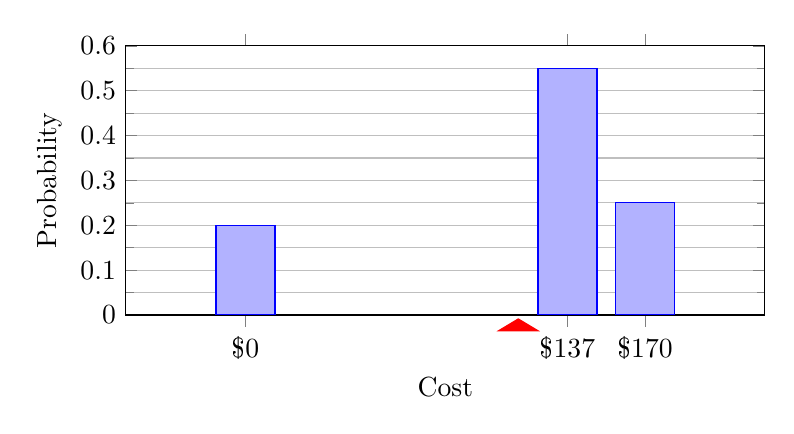
\begin{tikzpicture}
\FPset\expectedx{4.987} %chktex 36
\FPset\expectedy{-0.05} %chktex 36

\FPeval\expectedwidth{clip(0.25)} %chktex 36
\FPeval\expectedheight{clip(0.15)} %chktex 36

\FPeval\aptx{clip(\expectedx-\expectedwidth)} %chktex 36
\FPeval\apty{clip(\expectedy-\expectedheight)} %chktex 36

\FPeval\bptx{clip(\expectedx)} %chktex 36
\FPeval\bpty{clip(\expectedy)} %chktex 36

\FPeval\cptx{clip(\expectedx+\expectedwidth)} %chktex 36
\FPeval\cpty{clip(\expectedy-\expectedheight)} %chktex 36

\begin{axis}[
height=5.0cm,
width=0.8\textwidth,
enlarge x limits=0.3,
ymajorgrids=true,
minor y tick num=1,
yminorgrids=true,
ylabel={Probability},
xlabel={\variable{Cost}},
bar width=0.75cm,
%symbolic x coords={\$0, \$137, \$170},
ybar,
ymin=0,
ymax=0.6,
ytick={0,0.1,...,1},
xtick=data,
xticklabel style={/pgf/number format/.cd,fixed,precision=0},
xticklabel=\$\pgfmathprintnumber{\tick},
]
\addplot+
coordinates
{
(0, 0.2)
(137, 0.55)
(170, 0.25)
};
%\draw[red] (axis cs: 117.58,0) -- (axis cs: 117.58, 0.1);
\end{axis}
\filldraw[red] (\aptx,\apty) -- (\bptx, \bpty) -- (\cptx,\cpty) -- cycle;
\end{tikzpicture}
\end{center}
\end{example}
\end{frame}

\begin{frame}
\begin{block}{Expected Value Of A Discrete Random Variable}
If $X$ takes outcomes $x_1$, \ldots, $x_k$ with probabilities $\prob{X=x_1}$, \ldots, $\prob{X=x_k}$, the expected value of $X$ is:
\begin{equation*}
\begin{aligned}
E(X) &= x_1\cdot\prob{X=x_1} + x_2\cdot\prob{X=x_2} + \cdots + x_k\cdot\prob{X=x_k} \\
&= \sum_{i=1}^{k} x_i\cdot\prob{X=x_i}
\end{aligned}
\end{equation*}\pause
\end{block}

\begin{note}
The Greek letter $\mu$ is sometimes used in place of $E(X)$.
\end{note}
\end{frame}

\begin{frame}
\begin{example}
In American Roulette, a wheel with 38 numbered spaces is spun. There are 18 red spaces, 18 black spaces, and 2 green spaces.

\only<1 | handout:0>{%
\begin{center}
\vspace{8.65mm}
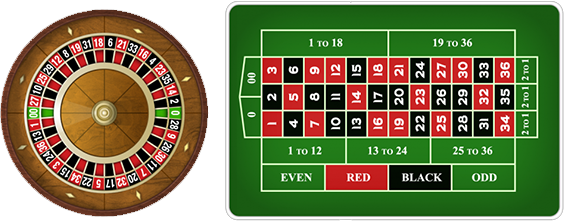
\includegraphics[scale=0.6]{American_roulette.png}
\vspace{8.65mm}
\end{center}
}
\only<2->{%
\vspace{1mm}
In one possible bet, the players bet \$1 on a single number. If that number is spun on the wheel, then they receive \$36. Otherwise, they lose their \$1.\pause\pause

\vspace{1mm}
If $X$ is the net winnings, then the probability distribution is:
\begin{center}
\begin{tabular}{lccc} \hline
$i$ & 1 & 2 & Total \\\hline
$x_i$ & \$35 & -\$1 & -- \\
$\prob{X=x_i}$ & $\dfrac{1}{38}$ & $\dfrac{37}{38}$ & 1\\[2mm]\hline
\end{tabular}
\end{center}\pause

The expected value of $X$ is:

\vspace{-2mm}
\begin{equation*}
\begin{aligned}
E(X) &= x_1\cdot\prob{X=x_1} + x_2\cdot\prob{X=x_2} \\\pause
&= \$35\cdot\dfrac{1}{38} + -\$1\cdot\dfrac{37}{38} \pause = \$0.9211 - \$0.9737 \pause \approx -\$0.053
\end{aligned}
\end{equation*}\pause

\vspace{-3mm}
On \emph{average}, the player will lose 5.3 cents per bet.
}
\end{example}
\end{frame}

\begin{frame}
\begin{example}
Suppose an individual has a 0.242\% risk of dying during the next year.

\vspace{1mm}
An insurance company charges \$275 for a life-insurance policy that pays \$100,000 death benefit.

\vspace{1mm}
\question{What is the expected value for the person buying the insurance?}\pause
\answer{%
The probabilities distribution is:
\begin{center}
\begin{tabular}{lrrr} \hline
$i$ & 1 & 2  & Total\\ \hline
$x_i$ &  \$99,725 & -\$275 & -- \\
$\prob{X=x_i}$ & 0.00242 & 0.99758 & 1.0\\\hline
\end{tabular}
\end{center}\pause

\vspace{-2mm}
The expected value is:

\vspace{-3mm}
\begin{equation*} 
\begin{aligned}
E(X) &= x_1\cdot\prob{X=x_1} + x_2\cdot\prob{X=x_2} \\\pause
&= \$99,725\cdot 0.00242 -\$275\cdot0.99758 \pause
= -\$33
\end{aligned}
\end{equation*}
\vspace{-3mm}
}
\end{example}\pause
\begin{note}\small
It makes sense that an insurance policy would have a negative expected value, otherwise the insurance company couldn't stay in business.
\end{note}
\end{frame}

\begin{frame}
\begin{example}
A company estimates that 0.7\% of their products will fail, with a replacement cost of \$350, after the original warranty period but within 2 years of the purchase. 

\vspace{1mm}
\question{If they offer a 2 year extended warranty for \$48, what is the company's expected value?}\pause
\answer{%
The probabilities and values for the two outcomes are:
\begin{center}
\begin{tabular}{lrrr} \hline
$i$ & 1 & 2 & Total \\\hline
$x_i$ & -\$302 & \$48 & -- \\
$\prob{X=x_i}$ & 0.007 & 0.993 & 1.0\\\hline 
\end{tabular}
\end{center}\pause
The expected value is:
\vspace{-2mm}
\begin{equation*} 
\begin{aligned}
E(X) &= x_1\cdot\prob{X=x_1} + x_2\cdot\prob{X=x_2} \\\pause
& =  -\$302\cdot 0.007 + \$48\cdot0.993 = \$45.55 \pause
= -\$33
\end{aligned}
\end{equation*}
\pause

\vspace{-4mm}
The company makes, on average, \$45.55 for each extended warranty.
}
\end{example}
\end{frame}

\begin{frame}
\begin{note}
If you ran the university bookstore in Example~\ref{bookstore}, then not only would you want to know your expected revenue, but also how much variability there is in your revenue.
\end{note}\pause

\begin{block}{General Variance Formula}
If $X$ takes outcomes $x_1$, \ldots, $x_k$ with probabilities $\prob{X=x_1}$, \ldots, $\prob{X=x_k}$ and expected value $\mu=E(x)$, then the variance of $X$, denoted by $Var(X)$ or the symbol $\sigma^2$, is:
\begin{equation*}
\begin{aligned}
\sigma^2 &= {(x_1 - \mu)}^2\cdot\prob{X=x_1} + \cdots + {(x_2 - \mu)}^2\cdot\prob{X=x_2} \\
&= \sum_{j=1}^{k} {(x_j - \mu)}^2\cdot\prob{X=x_j}
\end{aligned}
\end{equation*}
The standard deviation of $X$, denoted $\sigma$, is the square root of the variance.\ i.e.\ $\sigma = \sqrt{\sigma^2}$
\end{block}
\end{frame}

\FPset\xione{0.00} %chktex 36
\FPset\xitwo{137.00} %chktex 36
\FPset\xithree{170.00} %chktex 36
\FPset\Pxione{0.20} %chktex 36
\FPset\Pxitwo{0.55} %chktex 36
\FPset\Pxithree{0.25} %chktex 36
\FPeval\Ptimesxione{round(\xione*\Pxione:2)} %chktex 36
\FPeval\Ptimesxitwo{round(\xitwo*\Pxitwo:2)} %chktex 36
\FPeval\Ptimesxithree{round(\xithree*\Pxithree:2)} %chktex 36
\FPeval\expectedvalue{round(\Ptimesxione+\Ptimesxitwo+\Ptimesxithree:2)} %chktex 36
\FPeval\xionemu{round(\xione-\expectedvalue:2)} %chktex 36
\FPeval\xitwomu{round(\xitwo-\expectedvalue:2)} %chktex 36
\FPeval\xithreemu{round(\xithree-\expectedvalue:2)} %chktex 36
\FPeval\xionemusquared{round(\xionemu*\xionemu:2)} %chktex 36
\FPeval\xitwomusquared{round(\xitwomu*\xitwomu:2)} %chktex 36
\FPeval\xithreemusquared{round(\xithreemu*\xithreemu:2)} %chktex 36
\FPeval\finalone{round(\xionemusquared*\Pxione:2)} %chktex 36
\FPeval\finaltwo{round(\xitwomusquared*\Pxitwo:2)} %chktex 36
\FPeval\finalthree{round(\xithreemusquared*\Pxithree:2)} %chktex 36
\FPeval\variance{round(\finalone+\finaltwo+\finalthree:2)} %chktex 36
\FPeval\stddev{round(root(2,\variance):2)} %chktex 36

\begin{frame}
\begin{example}
Let us find the expected value of the bookstore in Example~\ref{bookstore}.\pause

\vspace{1mm}
It is useful to construct a table to hold the computations:

\vspace{-5mm}
\begin{center}
\scalebox{0.96}{%
\begin{tabular}{lrrrrl}\cline{1-5}
\visible<2->{$i$ & 1 & 2 & 3 & Total &} \\\cline{1-5}
\visible<3->{$x_i$ & \$\xione & \$\xitwo & \$\xithree & -- &}  \\
\visible<4->{$\prob{x=x_i}$ & \Pxione & \Pxitwo & \Pxithree & -- &}\\
\visible<5->{$x_i\cdot\prob{X=x_i}$ & \Ptimesxione & \Ptimesxitwo & \Ptimesxithree & \expectedvalue &} \visible<6->{$= \mu$} \\
\visible<7->{$x_i-\mu$ & \xionemu & \xitwomu & \xithreemu & --} \\
\visible<8->{${(x_i-\mu)}^2$ & \xionemusquared & \xitwomusquared & \xithreemusquared & --} \\
\visible<9->{${(x_i-\mu)}^2\cdot\prob{X=x_i}$ & \finalone & \finaltwo & \finalthree & \variance &} \visible<10->{$=\sigma^2$} \\\cline{1-5}
\end{tabular}
}
\end{center}

\vspace{-1mm}
\visible<11->{The variance of $X$ is $\sigma^2=\variance$ and so the standard deviation is $\sigma=\sqrt{\variance}=\$\stddev$.}

\vspace{1mm}
\visible<12->{So, on average, we can expect a variability of revenue of around \$$\stddev$ per student.}
\end{example}
\end{frame}

\FPset\xione{0.00} %chktex 36
\FPset\xitwo{159.00} %chktex 36
\FPset\xithree{200.00} %chktex 36
\FPset\Pxione{0.15} %chktex 36
\FPset\Pxitwo{0.25} %chktex 36
\FPset\Pxithree{0.60} %chktex 36
\FPeval\Ptimesxione{round(\xione*\Pxione:2)} %chktex 36
\FPeval\Ptimesxitwo{round(\xitwo*\Pxitwo:2)} %chktex 36
\FPeval\Ptimesxithree{round(\xithree*\Pxithree:2)} %chktex 36
\FPeval\expectedvalue{round(\Ptimesxione+\Ptimesxitwo+\Ptimesxithree:2)} %chktex 36
\FPeval\xionemu{round(\xione-\expectedvalue:2)} %chktex 36
\FPeval\xitwomu{round(\xitwo-\expectedvalue:2)} %chktex 36
\FPeval\xithreemu{round(\xithree-\expectedvalue:2)} %chktex 36
\FPeval\xionemusquared{round(\xionemu*\xionemu:2)} %chktex 36
\FPeval\xitwomusquared{round(\xitwomu*\xitwomu:2)} %chktex 36
\FPeval\xithreemusquared{round(\xithreemu*\xithreemu:2)} %chktex 36
\FPeval\finalone{round(\xionemusquared*\Pxione:2)} %chktex 36
\FPeval\finaltwo{round(\xitwomusquared*\Pxitwo:2)} %chktex 36
\FPeval\finalthree{round(\xithreemusquared*\Pxithree:2)} %chktex 36
\FPeval\variance{round(\finalone+\finaltwo+\finalthree:2)} %chktex 36
\FPeval\stddev{round(root(2,\variance):2)} %chktex 36

\begin{frame}
\begin{example}
The bookstore also offers a chemistry textbook for \$159 with a supplement for \$41. From past expereince, they know about 25\% of chemistry students just buy the textbook while 60\% buy both.\pause

\vspace{1mm} Let us construct the same type of table:
\vspace{-5mm}
\begin{center}
\scalebox{0.96}{%
\begin{tabular}{lrrrrl}\cline{1-5}
\visible<2->{$i$ & 1 & 2 & 3 & Total &} \\\cline{1-5}
\visible<3->{$x_i$ & \$\xione & \$\xitwo & \$\xithree & -- &}  \\
\visible<4->{$\prob{x=x_i}$ & \Pxione & \Pxitwo & \Pxithree & -- &}\\
\visible<5->{$x_i\cdot\prob{X=x_i}$ & \Ptimesxione & \Ptimesxitwo & \Ptimesxithree & \expectedvalue &} \visible<6->{$= \mu$} \\
\visible<7->{$x_i-\mu$ & \xionemu & \xitwomu & \xithreemu & --} \\
\visible<8->{${(x_i-\mu)}^2$ & \xionemusquared & \xitwomusquared & \xithreemusquared & --} \\
\visible<9->{${(x_i-\mu)}^2\cdot\prob{X=x_i}$ & \finalone & \finaltwo & \finalthree & \variance &} \visible<10->{$=\sigma^2$} \\\cline{1-5}
\end{tabular}
}
\end{center}

\vspace{-1mm}
\visible<11->{The variance of $X$ is $\sigma^2=\variance$ and so the standard deviation is $\sigma=\sqrt{\variance}=\$\stddev$.}

\vspace{1mm}
\visible<12->{So, on average, we can expect a variability of revenue of around \$$\stddev$ per student.}
\end{example}
\end{frame}

\begin{frame}
\begin{example}\label{john travels}
\vspace{-2mm}%beamer bug: extra space is added when a label is used, so this is to make this slide and the next look the same
John travels to work five days a week.\pause

\vspace{1mm}
We will use:
\begin{itemize}
\item $X_1$ to represent his travel time on Monday
\item $X_2$ to represent his travel time on Tuesday
\item $X_3$ to represent his travel time on Wednesday
\item $X_4$ to represent his travel time on Thursday
\item $X_5$ to represent his travel time on Friday
\end{itemize}\pause
His total travel time for the week is the sum of the daily five values:

\vspace{-3mm}
\begin{equation*}
W = X_1+X_2+X_3+X_4+X_5
\end{equation*}
\end{example}\pause

\begin{note}
By breaking the week into the individual days we can better understand the source of each randomness and is useful for modeling $W$.
\end{note}
\end{frame}

\begin{frame}
\begin{example}
It takes John an average of $E(X_i)=18$ minutes each day to commute to work.\pause

\vspace{1mm}
To find the expected value of his average commute times for the week we can sum the expected time for each day:

\vspace{-3mm}
\begin{equation*}
\begin{aligned}
E(W) &= E(X_1+X_2+X_3+X_4+X_5) \\
&= E(X_1)+E(X_2)+E(X_3)+E(X_4)+E(X_5) \\
&= 18 + 18 + 18 + 18 + 18 \\
&= 90~\text{minutes}
\end{aligned}
\end{equation*}\pause

\vspace{1mm}
\question{Would you be surprised if John's weekly commute wasn't exactly 90 minutes long?}\pause
\answer{There is always some variability with probabilities, so we can reasonably expect his commute to be a bit different from 90 minutes.}
\end{example}
\end{frame}

\begin{frame}
\begin{example}\label{elena ebay}
\vspace{-2mm}%beamer bug: extra space is added when a label is used, so this is to make this slide and the next look the same
Elena is selling a TV on eBay and plans to use the money to buy a toaster oven.\pause

\vspace{1mm}
Let $X$ represent the profit for selling the TV and $Y$ represent the cost of the toaster oven.\pause

\vspace{1mm}
\question{What equation represents the net change in Elena's eBay account?}\pause
\answer{The net change is money earned minus money spent: $X-Y$.}\pause

\vspace{1mm}
Based on past auctions, Elena figures she should expect to get about \$175 on the TV and pay about \$23 fo the toaster oven.\pause

\vspace{1mm}
\question{In total, how much should she expect to make or spend?}\pause
\answer{%
\begin{equation*}
E(X-Y) 
= E(X) - E(Y) \pause
= 175-23 \pause
=152 
\end{equation*}\pause
So, she should expect to make about \$152.
}
\end{example}
\end{frame}

\begin{frame}
\begin{definition}
A \textbf{linear combination} of two random variables $X$ and $Y$ is

\vspace{-3mm}
\begin{equation*}
aX+bY
\end{equation*}

\vspace{-2mm}
where $a$ and $b$ are some fixed and known numbers.
\end{definition}\pause

\begin{example}
In Example~\ref{elena ebay}, Elena's net change is the linear combination

\vspace{-3mm}
\begin{equation*}
1\cdot X + (-1)\cdot Y
\end{equation*}
\end{example}\pause

\begin{example}
In Example~\ref{john travels}, John's weekly commute time is the linear combination 

\vspace{-3mm}
\begin{equation*}
1\cdot X_1+1\cdot X_2+1\cdot X_3+1\cdot X_4+1\cdot X_5
\end{equation*}
\end{example}\pause

\begin{block}{Expected Value of Linear Combinations of Random Variables}
If $X$ and $Y$ are random variables, then

\vspace{-3mm}
\begin{equation*}
E(aX+bY) = a\cdot E(X) + b\cdot E(Y)
\end{equation*}
\end{block}
\end{frame}

\begin{frame}
\begin{example}
Leonard has invested \$6000 in Caterpiller Inc. (CAT) and \$2000 in Exxon Mobile Corp. (XOM).\pause

\vspace{1mm}
\begin{itemize}
\item $X$ represents the change in Caterpiller's stock next month, and 
\item $Y$ represents the change in Exxon Mobile's stock next month
\end{itemize}\pause

\question{What is the equation describing how much Leonard will make or lose next month?}\pause
\answer{%
\vspace{-6mm}
\begin{equation*}
\$6000\cdot X + \$2000\cdot Y
\end{equation*}
}\pause

\vspace{-4mm}
Caterpillar piller stock has recently been rising at 2.0\% and Exxon Mobil's at 0.2\% per month.\pause

\vspace{1mm}
\question{What is the expected change in Leonard's stock portfolio?}\pause
\answer{%

\vspace{-6mm}
\begin{equation*}
\begin{aligned}
E(\$6000\cdot X + \$2000\cdot Y) 
&=\$6000\cdot E(X) + \$2000\cdot Y \\\pause
&=\$6000\cdot 0.02 + \$2000\cdot 0.002 \pause
=\$124
\end{aligned}
\end{equation*}
}\pause

\vspace{-4mm}
\question{Would it be surprising to learn Leonard actually had a loss this month?}\pause
\answer{\small While stocks tend to rise over time, they are often volatile in the short term.}

\end{example}
\end{frame}

\begin{frame}
\begin{block}{Variability of Linear Combinations of Random Variables}
The variance of a linear combination is

\vspace{-3mm}
\begin{equation*}
Var(aX+bY) = a^2\cdot Var(X) + b^2\cdot Var(y)
\end{equation*}
\end{block}\pause

\begin{note}
This formula only works if $X$ and $Y$ are independent random variables.
\end{note}\pause

\begin{note}
Why the formula works and what happens if $X$ and $Y$ are dependent will be left to a dedicated probability course.
\end{note}\pause

\begin{note}
As usual, you can get the standard deviation by taking the square root of the variance.
\end{note}
\end{frame}

\begin{frame}
\begin{example}
Suppose John's daily commute has a standard deviation of 4 minutes.

\vspace{1mm}
\question{What is the uncertainty in his total weekly commute?}\pause
\answer{We start by noting that $Var(X_i) = \sigma^2 = 4^2 = 16$.\pause

\vspace{1mm}
Recall that that:

\vspace{-4mm}
\begin{equation*}
W=1\cdot X_1+1\cdot X_2+1\cdot X_3+1\cdot X_4+1\cdot X_5
\end{equation*}\pause

\vspace{-5mm}
So, 

\vspace{-4mm}
\begin{equation*}
\begin{aligned}
Var(W)
&= Var(1\cdot X_1+1\cdot X_2+1\cdot X_3+1\cdot X_4+1\cdot X_5) \\\pause
&= 1^2 \cdot 16 + 1^2 \cdot 16 + 1^2 \cdot 16 + 1^2 \cdot 16 + 1^2 \cdot 16 \\\pause
&= 80 \\\pause
\sigma &= \sqrt{Var(W)} \pause
 = \sqrt{80} \pause
 = 8.94
\end{aligned}
\end{equation*}

\vspace{-2mm}
The standard deviation for John's commute is about 9 minutes.
}\pause

\vspace{1mm}
\question{Is is reasonable to assume each daily commute is independent?}\pause
\answer{It depends on traffic patterns and what mode of transport John uses.}
\end{example}
\end{frame}

\begin{frame}
\begin{example}
It is reasonable to assume that an eBay auction for a TV is more or less independent from one for a toaster oven.\pause

\vspace{1mm}
Suppose that the standard deviation of TV auctions is \$25 and toaster oven auctions is \$8.

\vspace{1mm}
\question{What is the standard deviation of Elena's net gain?}\pause
\answer{%
Recall:
\begin{itemize}
\item \answernospacing{$X$ is the profit from the TV, so $Var(X) = 25^2 = 625$, and }\pause
\item \answernospacing{$Y$ is the cost of the toaster oven, so $Var(Y) = 8^2 = 64$.}\pause
\item \answernospacing{The linear combination is $X-Y=1\cdot X + (-1)\cdot Y$.}
\end{itemize}\pause

Then,
\vspace{-3mm}
\begin{equation*}
\begin{aligned}
Var(1\cdot X + (-1)\cdot Y) &= 1^2 \cdot Var(X) + {(-1)}^2\cdot  Var(Y) \\\pause
&= 1\cdot 625 + 1\cdot 64 \pause
= 689 \\\pause
\sigma &= \sqrt{689} \pause
= 26.25
\end{aligned}
\end{equation*}
The standard deviation for Elena's net gain is about \$26.25.
}
\end{example}
\end{frame}
\end{document}
